\documentclass[journal,12pt,twocolumn]{IEEEtran}

\usepackage{setspace}
\usepackage{gensymb}
\singlespacing
\usepackage[cmex10]{amsmath}

\usepackage{amsthm}

\usepackage{mathrsfs}
\usepackage{txfonts}
\usepackage{stfloats}
\usepackage{bm}
\usepackage{cite}
\usepackage{cases}
\usepackage{subfig}

\usepackage{longtable}
\usepackage{multirow}

\usepackage{enumitem}
\usepackage{mathtools}
\usepackage{steinmetz}
\usepackage{tikz}
\usepackage{circuitikz}
\usepackage{verbatim}
\usepackage{tfrupee}
\usepackage[breaklinks=true]{hyperref}
\usepackage{graphicx}
\usepackage{tkz-euclide}

\usetikzlibrary{calc,math}
\usepackage{listings}
    \usepackage{color}                                            %%
    \usepackage{array}                                            %%
    \usepackage{longtable}                                        %%
    \usepackage{calc}                                             %%
    \usepackage{multirow}                                         %%
    \usepackage{hhline}                                           %%
    \usepackage{ifthen}                                           %%
    \usepackage{lscape}     
\usepackage{multicol}
\usepackage{chngcntr}

\DeclareMathOperator*{\Res}{Res}

\renewcommand\thesection{\arabic{section}}
\renewcommand\thesubsection{\thesection.\arabic{subsection}}
\renewcommand\thesubsubsection{\thesubsection.\arabic{subsubsection}}

\renewcommand\thesectiondis{\arabic{section}}
\renewcommand\thesubsectiondis{\thesectiondis.\arabic{subsection}}
\renewcommand\thesubsubsectiondis{\thesubsectiondis.\arabic{subsubsection}}


\hyphenation{op-tical net-works semi-conduc-tor}
\def\inputGnumericTable{}                                 %%

\lstset{
%language=C,
frame=single, 
breaklines=true,
columns=fullflexible
}
\begin{document}

\newcommand{\BEQA}{\begin{eqnarray}}
\newcommand{\EEQA}{\end{eqnarray}}
\newcommand{\define}{\stackrel{\triangle}{=}}
\bibliographystyle{IEEEtran}
\raggedbottom
\setlength{\parindent}{0pt}
\providecommand{\mbf}{\mathbf}
\providecommand{\pr}[1]{\ensuremath{\Pr\left(#1\right)}}
\providecommand{\qfunc}[1]{\ensuremath{Q\left(#1\right)}}
\providecommand{\sbrak}[1]{\ensuremath{{}\left[#1\right]}}
\providecommand{\lsbrak}[1]{\ensuremath{{}\left[#1\right.}}
\providecommand{\rsbrak}[1]{\ensuremath{{}\left.#1\right]}}
\providecommand{\brak}[1]{\ensuremath{\left(#1\right)}}
\providecommand{\lbrak}[1]{\ensuremath{\left(#1\right.}}
\providecommand{\rbrak}[1]{\ensuremath{\left.#1\right)}}
\providecommand{\cbrak}[1]{\ensuremath{\left\{#1\right\}}}
\providecommand{\lcbrak}[1]{\ensuremath{\left\{#1\right.}}
\providecommand{\rcbrak}[1]{\ensuremath{\left.#1\right\}}}
\theoremstyle{remark}
\newtheorem{rem}{Remark}
\newcommand{\sgn}{\mathop{\mathrm{sgn}}}
\providecommand{\abs}[1]{\vert#1\vert}
\providecommand{\res}[1]{\Res\displaylimits_{#1}} 
\providecommand{\norm}[1]{\lVert#1\rVert}
%\providecommand{\norm}[1]{\lVert#1\rVert}
\providecommand{\mtx}[1]{\mathbf{#1}}
\providecommand{\mean}[1]{E[ #1 ]}
\providecommand{\fourier}{\overset{\mathcal{F}}{ \rightleftharpoons}}
%\providecommand{\hilbert}{\overset{\mathcal{H}}{ \rightleftharpoons}}
\providecommand{\system}{\overset{\mathcal{H}}{ \longleftrightarrow}}
	%\newcommand{\solution}[2]{\textbf{Solution:}{#1}}
\newcommand{\solution}{\noindent \textbf{Solution: }}
\newcommand{\cosec}{\,\text{cosec}\,}
\providecommand{\dec}[2]{\ensuremath{\overset{#1}{\underset{#2}{\gtrless}}}}
\newcommand{\myvec}[1]{\ensuremath{\begin{pmatrix}#1\end{pmatrix}}}
\newcommand{\mydet}[1]{\ensuremath{\begin{vmatrix}#1\end{vmatrix}}}
\numberwithin{equation}{subsection}
\makeatletter
\@addtoreset{figure}{problem}
\makeatother
\let\StandardTheFigure\thefigure
\let\vec\mathbf
\renewcommand{\thefigure}{\theproblem}
\def\putbox#1#2#3{\makebox[0in][l]{\makebox[#1][l]{}\raisebox{\baselineskip}[0in][0in]{\raisebox{#2}[0in][0in]{#3}}}}
     \def\rightbox#1{\makebox[0in][r]{#1}}
     \def\centbox#1{\makebox[0in]{#1}}
     \def\topbox#1{\raisebox{-\baselineskip}[0in][0in]{#1}}
     \def\midbox#1{\raisebox{-0.5\baselineskip}[0in][0in]{#1}}
\vspace{3cm}
\title{AI1103-Assignment 1}
\author{Name: Kethavath Praneeth Nayak, Roll Number: CS20BTECH11025}
\maketitle
\newpage
\bigskip
\renewcommand{\thefigure}{\theenumi}
\renewcommand{\thetable}{\theenumi}
Download all python codes from 
\begin{lstlisting}
https://github.com/PraneethNyk/Assignment_1-AI1103/blob/main/ASSIGNMENT_1.py
\end{lstlisting}
%
and latex codes from 
%
\begin{lstlisting}
https://github.com/PraneethNyk/Assignment_1-AI1103/blob/main/ASSIGNMENT_1.tex
\end{lstlisting}
\section*{Question}
Ten cards numbered 1 to 10 are placed in
a box, mixed up thoroughly and then one
card is drawn randomly. If it is known that
the number on the drawn card is more than
3, what is the probability that it is an even
number?
\section*{Solution}
The set of sample space which contains cards numbered from 1 to 10 be 
\begin{align}
S \in \{1,2,3,4,5,6,7,8,9,10\}
\end{align}
Now probability of picking a random card from ten cards is be $Pr(x)$. Then,
\begin{align}
Pr(x\in S )=\frac{1}{10}
\end{align}
Let the Set of Even numbered cards be $E$ and Set of cards numbered greater than 3 is $A$.
and we know that the set of even numbers from 1 to 10 is \{2,4,6,8,10\} . Then,
\begin{align}
E \in \{2,4,6,8,10\}    
\end{align}
Now here, The Set of numbers greater than 3 
is \{4,5,6,7,8,9,10\}. Then,
\begin{align}
    A \in \{4,5,6,7,8,9,10\}
\end{align}
\begin{align}
    Pr(A)=\frac{No.\; of\; elements\; in\; (A).}{Number\; of\; cards.}
\end{align}
\begin{align}
\label{eq1}
    Pr(A)=\frac{7}{10}=0.7
\end{align}
Now, the favoured outcomes are set of $EA$ and 
Here the set $EA$ contains the cards which are even and numbered greater than 3.
\begin{align}
    Pr(EA)=\frac{No.\; of\; elements\; in\; E A.}{Number\; of\;cards.}
\end{align}
\begin{align}
   Now , Pr(EA) = Pr(4)+Pr(6)+Pr(8)+Pr(10)
\end{align}
\begin{align}
\label{eq2}
     Pr(EA) =\frac{4}{10}=0.4 
\end{align}
The probability that the card drawn is even number which is greater than 3 is
\begin{align}
    Pr(E|A)=\frac{Pr(EA)}{Pr(A)}
\end{align}
Now,using (\ref{eq1}) and (\ref{eq2}). 
\begin{align}
  (\because Pr(EA)=0.4\; and \; Pr(A)=0.7)  
\end{align}
\begin{align}
And, Pr(E|A)=\frac{Pr(EA)}{Pr(A)}
\end{align}
\begin{align}
=\frac{0.4}{0.7}
\end{align}
\begin{align}
\therefore Pr(E|A)=\frac{4}{7}    
\end{align}
\begin{align}
\therefore Pr(E|A)=0.5714285714285714    
\end{align}
\begin{figure}
   \caption{Plots of Theoritical versus expermental probabilities}
    \centering
    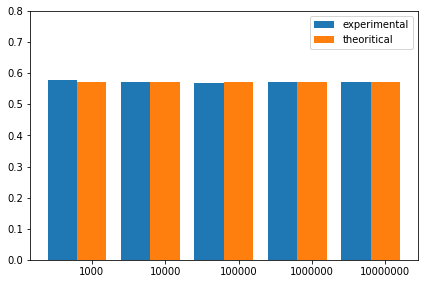
\includegraphics[width=\columnwidth]
    {Figure.png}
\end{figure}

\end{document}